\chapter{Additional Figures}
\label{ap:addFig}

\begin{itemize}
	\item integrated autocorrelation time, cite Ulli Wolf \cite{UwerrM} pyhton and matlab
	\item acceptance rate for one D and multi D, cite roberts
\end{itemize}

\chapter{Correlation Structure}
\label{ap:Correlatation}
In the book Gaussian Markov Random Fields~\cite{rue2005gaussian}, Rue and Held demonstrate that a strong correlation between the hyper-parameter $\mu$ and the latent field $\bm{x}$ can significantly slow down convergence when using samplers, in particularly Gibbs samplers. 
They consider the hierarchical model

\begin{subequations}
\begin{align}
\mu &\sim \mathcal{N}(0, 1) \\
\bm{x} | \mu &\sim \mathcal{N}(\mu \bm{1}, \bm{Q}^{-1}),
\end{align}
\label{eq:rueMod}
\end{subequations}

and apply a Gibbs sampler based on the full conditional distributions
\begin{align}
	\mu^{(k)} | \bm{x}^{(k)} &\sim \mathcal{N} \left( \frac{\bm{1}^T \bm{Q} \bm{x}^{(k-1)}}{1 + \bm{1}^T \bm{Q} \bm{1}}, \, \left(1 + \bm{1}^T \bm{Q} \bm{1} \right)^{-1} \right) \\
	\bm{x}^{(k)} | \mu^{(k)} &\sim \mathcal{N}(\mu^{(k)} \bm{1}, \bm{Q}^{-1}).
\end{align}
As illustrated in Figure~\ref{fig:RueHeld}, when the sampler is restricted to steps only in the $\mu$-direction (horizontal axis) or the $\bm{x}$-direction (vertical axis), it requires many iterations to adequately explore the parameter space. 
This inefficiency arises from the high correlation between $\mu$ and $\bm{x}$, visible in Figure~\ref{fig:RueHeld} as a 'squeeze' of the distribution.
\begin{figure}[ht!]
	\centering
	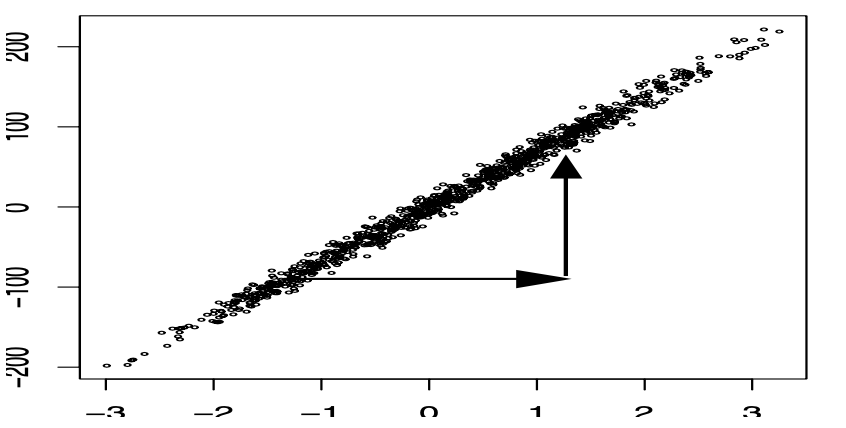
\includegraphics[width = \textwidth]{Figures/RueHeldBookFig.png}
	\caption[Correlation structure in between parameters and hyper-parameters]{The figure taken from~\cite[Figure 4.1 (b)]{rue2005gaussian}, shows samples from a marginal chain for $\mu$ and $\bm{1}^T \bm{Q} \bm{x}^{(k)}$ over 1000 iterations, based on the hierarchical model in Eq.~\ref{eq:rueMod}, with an autoregressive process encoded in $\bm{Q}$. The algorithm updates $\mu$ and $\bm{x}$ successively from their full conditional distributions. The plot displays $(\mu^{(k)}, \bm{1}^T \bm{Q} \bm{x}^{(k)})$, with $\mu^{(k)}$ on the horizontal axis and $\bm{1}^T \bm{Q} \bm{x}^{(k)}$ on the vertical axis. The slow mixing and convergence of $\mu$ result from its strong dependence on $\bm{1}^T \bm{Q} \bm{x}^{(k)}$, while the sampler permits only axis-aligned (horizontal and vertical) and does not allow diagonal moves, as illustrated by the arrows.}
	\label{fig:RueHeld}
\end{figure}

A solution to the slow mixing problem is to update $(\mu, \bm{x})$ jointly.
Since here $\mu$ is one dimensional, effectively only marginal density of $\mu$ is needed.
\begin{align}
	\mu^{\star}  &\sim q (\mu^{\star}|	\mu^{(k-1)} ) \\
	\bm{x}^{(k)} | \mu^{\star} &\sim \mathcal{N} (	\mu^{\star}\bm{1}, \bm{Q}^{-1}) 
\end{align}
With a simple MCMC algorithm targeting  $ \mu$ one can explore the sample space efficiently and only draw a corresponding sample for $\bm{x}$ from its full conditional once, for instance, the proposal $\mu^{\star}$ has been accepted.

\chapter{Mesure theroy}
\label{ch:Mesure}
Recall the probability space $(\Omega, \mathcal{F}, \mathbb{P})$, where $\Omega$ denotes the sample space, and $\mathcal{F}$ is a collection of countable subsets $\{ A_n \}_{n \in \mathbb{N}}$ of $\Omega$. Each $A_n \subseteq \Omega$ is called an event, and a map $\mathbb{P} : \mathcal{F} \rightarrow \mathbb{R}$ is referred to as a measure.
In the following, we describe the conditions required for $\mathcal{F}$ to be a $\sigma$-algebra, and for $\mathbb{P}$ to qualify as a probability measure.
We refer to \cite{lawler2016notes} \cite{kopp2004measintprob} for further reading.

\section{probailty measure}
For a probability measure, we require:
\begin{itemize}
	\item $\mathbb{P}(\Omega) = 1$ and $\mathbb{P}(\emptyset) = 0$
	\item $\mathbb{P}(A) \in [0,1]$
	\item $\mathbb{P}(\bigcup_{j \in \mathbb{N}} A_j )= \sum_{j \in \mathbb{N}}  \mathbb{P}(A_j)$ if we have pairwise disjoint sets or $A_i \cap A_j = \emptyset$ for $i \neq j $
\end{itemize}
In other words, the probability assigned to the entire sample space must be equal to one, $\mathbb{P}(\Omega) = 1$, and the probability of the empty set must be zero, $\mathbb{P}(\emptyset) = 0$. For any subset $A \subseteq \Omega$, the probability $\mathbb{P}(A)$ must lie between zero and one, i.e., $\mathbb{P}(A) \in [0,1]$.
If e.g. two subsets $A$ and $B$ are disjoint (i.e., $A \cap B = \emptyset$), then the probability of their union satisfies $\mathbb{P}(A \cup B) = \mathbb{P}(A) + \mathbb{P}(B)$.
This property must also hold for a countable sequence of disjoint sets $\{A_j\}_{j \in \mathbb{N}}$, such that $\mathbb{P}\left( \bigcup_{j \in \mathbb{N}} A_j \right) = \sum_{j \in \mathbb{N}} \mathbb{P}(A_j)$.

\section{$\sigma$-algebra}
A collections of subsets $\mathcal{F}$ is called $\sigma$-algebra if:
\begin{itemize}
	\item $\emptyset, \Omega \in \mathcal{F} $,
	\item if $A \in \mathcal{F} $ then $A^C \coloneqq A / \Omega \in \mathcal{F}$
	\item if $A_1 , A_2, \dots  \in \mathcal{F} $ then $ \bigcup_{j \in \mathbb{N}}  A_j \in  \mathcal{F}$
\end{itemize}
In other words, the empty set $\emptyset$ and the entire sample space $\Omega$ must always be elements of $\mathcal{F}$. If a set $A \in \mathcal{F}$, then its complement $A^C = \Omega \setminus A$ must also be in $\mathcal{F}$. 
If, in terms of a probability measure, we are able to assign a probability $\mathbb{P}(A)$ to an event $A$, we must also be able to assign a probability to the event “not $A$”, i.e., $\mathbb{P}(A^C)$.
Finally, if a countable collection of sets $A_1, A_2, \dots \in \mathcal{F}$, then their union $\bigcup_{j \in \mathbb{N}} A_j$ must also be in $\mathcal{F}$. These three properties define the requirements for $\mathcal{F}$ to be a $\sigma$-algebra.
